\section{Definition}

Blockchain is an innovative technology introduced by \textbf{Satoshi Nakamoto} in 2008 through his famous paper \href{https://bitcoin.org/bitcoin.pdf}{"Bitcoin: A Peer-to-Peer Electronic Cash System"} \cite{bitcoinSatoshi}. It is a revolutionary cryptography-based electronic payment system designed to overcome the imitations of traditional systems and promote decentralization.

\begin{remark}
Defined as "\textit{a Blockchain}," each block contains a cryptographic hash of the previous block, a timestamp and transaction data. This blockchain structure makes each block inextricably linked to the others, creating an immutable and transparent digital ledger.
\end{remark}

Blockchain's basic purpose is to act as a decentralized ledger, which means that transactions are recorded permanently and immutably without the need for a central authority. It also enables consensus to be maintained in a trust-free environment, allowing unknown and potentially untrusted participants to collaborate securely.

Trade Ledger is not that far back in the history of accounting evolution. Interestingly, the double-entry accounting system described in Luca Pacioli's book has origins dating back to the possible influence of the Muslim accounting practice implemented by the Venetians \cite{accountingBooks}. So yes, ledgers are not new at all!

Now that we understand the essence of blockchain technology and its historical roots, let us delve into the concepts of \textbf{Distributed Ledgers} and \textbf{Decentralized Ledgers}. Understanding these concepts is critical as they form the backbone of various blockchain implementations.

\section{Decentralized Ledgers}
A decentralized ledger is essentially a registry that is managed and updated by multiple parties without the need for a central authority. Imagine this ledger as a document shared among several participants, but instead of being controlled by a single entity, it is distributed over a peer-to-peer (P2P) network. In this network, each node has a copy of the ledger and can verify its transactions.

\textbf{\textcolor{Orange}{Strengths}}:
\begin{itemize}
\item \textbf{Enhanced Security}: Because there is no central point of control, decentralized ledgers are less vulnerable to cyber attacks.
\item \textbf{Transparency and Accountability}: All parties involved can see and verify transactions, promoting transparency and accountability.
\item \textbf{Trustless Environments}: No need to rely on intermediaries to verify transactions, creating a trustless environment.
\end{itemize}

\vspace{2cm}

\textbf{\textcolor{Orange}{Drawbacks}}:
\begin{itemize}
\item \textbf{Processing Speed}: Due to the consensus required by multiple parties, transactions can be slower than in centralized systems.
\item \textbf{Complexity of Implementation}: Multi-party coordination and agreement are required to effectively implement a decentralized ledger.
\item \textbf{High Costs}: Maintaining the network requires significant resources in terms of computing power and energy.
\end{itemize}

\section{Distributed Ledgers}

A distributed ledger is a ledger that is managed and updated by multiple parties and stored in multiple locations. Unlike a decentralized ledger, which is distributed over a peer-to-peer network, a distributed ledger operates over a distributed network, where each node in the network owns a copy of the ledger and can validate transactions.

\textbf{\textcolor{Orange}{Strengths}}:

\begin{itemize}
    \item \textbf{Enhanced Processing Speed}: Distributed ledgers can be faster than decentralized ledgers because they can process transactions in parallel.
    \item \textbf{Improved Scalability}: Being more scalable than decentralized ledgers, distributed ledgers can be expanded to accommodate more users and transactions.
    \item \textbf{Increased Flexibility}: Distributed ledgers can be more flexible than decentralized ledgers because they can be customized to meet specific needs.
\end{itemize}

\textbf{\textcolor{Orange}{Drawbacks}}:

\begin{itemize}
    \item \textbf{Potentially Lower Security}: Unlike decentralized ledgers, distributed ledgers may be less secure because there is a central control point that could be targeted by hackers.
    \item \textbf{Reduced Transparency and Accountability}: Some parts of the network may have more control over the ledger than others, reducing overall transparency and accountability.
    \item \textbf{Complexity and Management}: Distributed ledgers can be more complex and difficult to manage than decentralized ledgers because they require coordination and agreement among multiple parties and multiple copies of the ledger.
\end{itemize}


\section{The Role of Trust and the Evolution of the Blockchain}

Trust plays a central role in understanding blockchain, going beyond mere technology and raising crucial philosophical and political questions concerning governance and the distribution of power.

Throughout history, philosophers and political theorists have examined different forms of social organization and the role of trust in institutions. From Plato to Hayek, perspectives vary widely, influencing our conceptions of power and trust.

The 2008 financial crisis acted as a catalyst for the adoption and development of blockchain and Bitcoin. The collapse of banks and financial institutions profoundly undermined trust in central institutions, pushing for greater decentralization and financial autonomy.

Moreover, blockchain does not simply represent a new technological invention, but rather an amalgamation of existing technologies that have been developed and refined over time. It is through the evolution of these technologies that blockchain has taken shape and begun to play a significant role in the digital landscape. To better understand this process, let us examine a rough timeline of key inventions:

\begin{figure}[htbp]
\centering
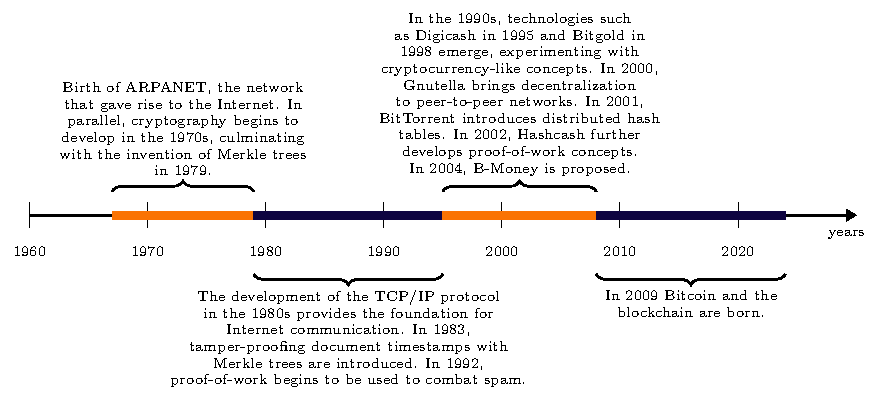
\includegraphics[width=1\textwidth]{tikz/chapter1 - Blockchain Timeline.pdf}
\caption{Blockchain Key Inventions Timeline}
\end{figure}